% !TeX root = ../main.tex
\documentclass[class=article]{standalone}

\begin{document}
\section*{Question 7}

Elle est ambiguë, prenons par exemple \lstinline{abaaba}.
Il est possible d'avoir l'arbre de dérivation suivante:

\begin{tikzpicture}
    [
    every leaf node/.style={draw,circle},
    sibling distance=1.5em, level distance=40pt]

    \tikzset{edge from parent/.style={draw, edge from parent path=
    {(\tikzparentnode) -- (\tikzchildnode)}}}
    \Tree 
    [.S 
        [.S
            a
            [.S
                $\epsilon$
            ]
            b
            [.S
                $\epsilon$
            ]
            a
        ]
        [.S
            a
            [.S
                $\epsilon$
            ]
            b
            [.S
                $\epsilon$
            ]
            a
        ]
    ]
\end{tikzpicture}

Mais, il est aussi possible d'avoir un autre arbre de dérivation, 
comme par exemple, celui-ci:


\begin{tikzpicture}
    [
    every leaf node/.style={draw,circle},
    sibling distance=1.5em, level distance=40pt]

    \tikzset{edge from parent/.style={draw, edge from parent path=
    {(\tikzparentnode) -- (\tikzchildnode)}}}
    \Tree 
    [.S 
        a
        [.S
            $\epsilon$
        ]
        b
        [.S
            a
            [.S
                $\epsilon$
            ]
            a
            [.S
                $\epsilon$
            ]
            b
        ]
        a
    ]
\end{tikzpicture}

\end{document}